\documentclass[12pt,letterpaper]{exam}
\usepackage[lmargin=1in,rmargin=1in,tmargin=1in,bmargin=1in]{geometry}
\usepackage{../style/exams}

% -------------------
% Course & Exam Information
% -------------------
\newcommand{\course}{MATH 141: Exam 2}
\newcommand{\term}{Fall ---\textsubscript{\textsubscript{2}} 2025}
\newcommand{\examdate}{10/24/2025}
\newcommand{\timelimit}{50 Minutes}

\setbool{hideans}{true} % Student: True; Instructor: False

\usepackage{cancel}
\newcommand{\myarc}[6]{\draw[#1] ({#2+#4*cos(#5)},{#3+#4*sin(#5)}) arc (#5:#6:#4)}

% -------------------
% Content
% -------------------
\begin{document}

\examtitle
\instructions{Write your name on the appropriate line on the exam cover sheet. This exam contains \numpages\ pages (including this cover page) and \numquestions\ questions. Check that you have every page of the exam. Answer the questions in the spaces provided on the question sheets. Be sure to answer every part of each question and show all your work. If you run out of room for an answer, continue on the back of the page --- being sure to indicate the problem number.} 
\scores
\bottomline
\newpage


% -------------------
% Questions
% -------------------
\begin{questions}

% Question 1
\newpage
\question[15] The approximation $\sqrt[4]{1 + x} \approx 1 + \dfrac{x}{4}$ for ``small'' $x$ is often used in Physics. Justify this approximation by finding the linearization of $f(x)= \sqrt[4]{1 + x}$ when $x= 0$. \pspace

\vsol{\itshape We know that the linearization of a function $f(x)$ at $x= a$ is given by\dots
	\[
	\ell(x)= f(a) + f'(a) \,\big(x - a \big)
	\]
We have $f(x)= \sqrt[4]{1 + x}= (1 + x)^{1/4}$ and $a= 0$, so that\dots
	\[
	\begin{aligned}
	f(0)&= \sqrt[4]{1 + x}= \sqrt[4]{1 + 0}= \sqrt[4]{1}= 1 \\[0.3cm]
	f'(x)&= \dfrac{1}{4} (1 + x)^{-3/4}= \dfrac{1}{4(1 + x)^{3/4}}= \dfrac{1}{4 \sqrt[4]{(1 + x)^3}} \\[0.3cm]
	f'(0)&= \dfrac{1}{4 \sqrt[4]{(1 + 0)^3}}= \dfrac{1}{4 \sqrt[4]{1}}= \dfrac{1}{4}
	\end{aligned}
	\]
Therefore, we have\dots
	\[
	\ell(x)= f(0) + f'(0) \,\big(x - 0 \big)= 1 + \dfrac{1}{4} \cdot x= 1 + \dfrac{4}{3}
	\]
Because $f(x) \approx \ell(x)$ when $x \approx 0$, we know that for ``small'' $x$, i.e. $x \approx 0$, that\dots
	\[
	\sqrt[4]{1 + x} \approx 1 + \dfrac{x}{4}
	\] \vfill

{\small Note. Generally, the approximation used in Physics is $\sqrt[n]{1 + x} \approx 1 + \dfrac{x}{n}$ for $n \geq 2$ when $x$ is `small'', i.e. $x \approx 0$.}
}



% Question 2
\newpage
\question Showing all your work, answer the following:
	\begin{parts}
	\part[5] Given that $(x + y)^6= x - y^3$, find $\dfrac{dy}{dx}$. \par\vspace{0.1cm}
	
	\wsol{\itshape\small
		\[
		\begin{gathered}
		(x + y)^6= x - y^3 \\[0.2cm]
		\dfrac{d}{dx} \left( (x + y)^6 \right) = \dfrac{d}{dx} (x - y^3) \\[0.2cm]
		6(x + y)^5 \cdot (1 + y')= 1 - 3y^2 \,y' \\[0.2cm]
		6(x + y)^5 + 6(x + y)^5 \, y' = 1 - 3y^2 \,y' \\[0.2cm]
		3y^2 \, y' + 6(x + y)^5 \, y' = 1 - 6(x + y)^5 \\[0.2cm]
		\big(3y^2 + 5(x + y)^4 \big) \, y' = 1 - 6(x + y)^5 \\[0.2cm]
		\boxed{\dfrac{dy}{dx}= \dfrac{1 - 6(x + y)^5}{3y^2 + 6(x + y)^5}} 
		\end{gathered}
		\]
	} \par\vspace{0.3cm}

	\part[5] Assuming that $x$ depends on time but $y$ \textit{does not}, differentiate the following expression with respect to time, $t$: \enskip $x^3 + y^4 - \sin(xy)$ \par\vspace{0.1cm}

	\wsol{\itshape\small Because $y$ does not vary with time, we know that $\tfrac{dy}{dt}= 0$. [So the derivative of any term depending only on $y$ is 0 as $\tfrac{d}{dt} f(y)= f'(y) \cdot \frac{dy}{dt}= 0$.] But then\dots
		\[
		\begin{gathered}
		\dfrac{d}{dt} \, (x^3 + y^4 - \sin(xy)) \\[0.2cm]
		3x^2 \,\dfrac{dx}{dt} + 0 - \cos(xy) \cdot \dfrac{d}{dt} (xy) \\[0.2cm]
		3x^2 \,\dfrac{dx}{dt} - \cos(xy) \cdot \left( \dfrac{dx}{dt} \,y + x \, \dfrac{dy}{dt} \right) \\[0.2cm]
		3x^2 \,\dfrac{dx}{dt} - \cos(xy) \cdot \left( \dfrac{dx}{dt} \,y + x \cdot 0 \right) \\[0.2cm]
		3x^2 \,\dfrac{dx}{dt} - y \cos(xy) \, \dfrac{dx}{dt}
		\end{gathered}
		\]
	} \par\vspace{0.3cm}

	\part[5] Assuming that \textit{both} $x$ and $y$ depend on time, differentiate the following expression with respect to time, $t$: \enskip $x^3 + y^3 - \sin(xy)$ \par\vspace{0.1cm}

	\wsol{\itshape\small
		\[
		\begin{gathered}
		\dfrac{d}{dt} \, (x^3 + y^3 - \sin(xy)) \\[0.2cm]
		3x^2 \,\dfrac{dx}{dt} + 3y^2 \,\dfrac{dy}{dt} - \cos(xy) \cdot \dfrac{d}{dt} (xy) \\[0.2cm]
		3x^2 \,\dfrac{dx}{dt} + 3y^2 \,\dfrac{dy}{dt} - \cos(xy) \cdot \left( \dfrac{dx}{dt} \,y + x \, \dfrac{dy}{dt} \right) 
		\end{gathered}
		\]
	}
	\end{parts}



% Question 3
\newpage
\question[15] Showing all your work, compute the following limits: \par\vspace{0.3cm}
	\begin{enumerate}[(a)]
	\item $\ds\lim_{x \to 0} \dfrac{x}{\arctan(x)}$ \pspace

	\wsol{%
		\[
		\lim_{x \to 0} \dfrac{x}{\arctan(x)} \stackrel{\text{L.H.}}{=} \lim_{x \to 0} \dfrac{\;\;1\;\;}{\;\;\tfrac{1}{1 + x^2}\;\;}= \lim_{x \to 0} (1 + x^2)= 1 + 0= 1
		\]
	} \par\vspace{0.3cm}\vfill

	\item $\ds\lim_{x \to \infty} \dfrac{\ln x}{\sqrt[3]{x}}$ \pspace

	\wsol{%
		\[
		\lim_{x \to \infty} \dfrac{\ln x}{\sqrt[3]{x}} \stackrel{\text{L.H.}}{=} \lim_{x \to \infty} \dfrac{\;\;\tfrac{1}{x}\;\;}{\tfrac{1}{3}\, x^{-2/3}}= \lim_{x \to \infty} \dfrac{3x^{2/3}}{x}= \lim_{x \to \infty} \dfrac{3}{x^{1/3}}= 0
		\]
	} \par\vspace{0.3cm}\vfill

	\item $\ds\lim_{x \to 0} (\cos x)^{-6/x^2}$ \pspace

	\wsol{%
		\[
		\begin{aligned}
		L&:= \lim_{x \to 0} (\cos x)^{-6/x^2} \\
		\ln L&= \lim_{x \to 0} \ln (\cos x)^{-6/x^2} \\
		\ln L&= \lim_{x \to 0} -\dfrac{6}{x^2} \ln(\cos x) \\
		\ln L&= \lim_{x \to 0} \dfrac{-6\ln(\cos x)}{x^2} \\
		\ln L&\stackrel{\text{L.H.}}{=} \lim_{x \to 0} \dfrac{-\dfrac{6}{\cos x} \cdot -\sin x}{2x} \\
		\ln L&= \lim_{x \to 0} \dfrac{3\sin x}{x \cos x} \\
		\ln L&\stackrel{\text{L.H.}}{=} \lim_{x \to 0} \dfrac{3\cos x}{\cos x + x (-\sin x)} \\
		\ln L&= \dfrac{3}{1 + 0} \\
		\ln L&= \dfrac{3}{1} \\
		e^{\ln L}&= e^3 \\
		L&= e^3
		\end{aligned}
		\]
	}
	\end{enumerate}



% Question 4
\newpage
\question[15] Find the point on curve $y= 4\sqrt{x}$ closest to the point $(10, 0)$. \par\vspace{0.1cm}

\vsol{\itshape We first create a sketch of the described problem. 
	\[
	\fbox{
	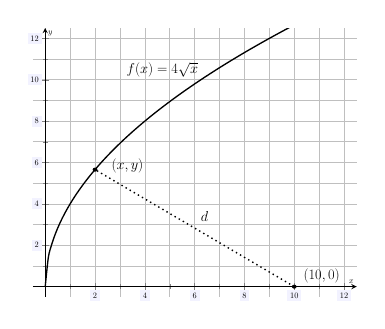
\begin{tikzpicture}[scale=0.60,every node/.style={scale=0.5}]
	\begin{axis}[
	grid=both,
	axis lines=middle,
	ticklabel style= {fill= blue!5!white},
	xmin= -0.5, xmax=12.5,
	ymin= -0.5, ymax=12.5,
	xtick= {0,2,...,12},
	ytick= {0,2,...,12},
	minor tick = {-10,-9,...,12},
	xlabel= \(x\), ylabel= \(y\)
	]
	\node at (4.7,10.5) {\LARGE$f(x)= 4 \sqrt{x}$};
	\addplot[thick, samples=100, smooth, domain= 0:12.5] ({x},{sqrt(16*x)});
	
	\node at (6.4,3.4) {\LARGE$d$};
	
	\node at (11.1,0.5) {\LARGE$(10, 0)$};
	\draw[fill=black] (10,0) circle (0.08);
	
	\node at (2+1.3,{4*sqrt(2)+0.2}) {\LARGE$(x, y)$};
	\draw[fill=black] (2,{4*sqrt(2)}) circle (0.08);
	
	\draw[line width=0.03cm,dotted] (10,0) -- (2,{4*sqrt(2)});
	\end{axis}
	\end{tikzpicture}
	}
	\]
We want to minimize the distance between any point $(x, y)$ on the curve $y= 4 \sqrt{x}$ and the point $(10, 0)$. We know that this distance is given by $d= \sqrt{(x - a)^2 + (y - b)^2}$. But $(a, b)= (10, 0)$, so we have $d= \sqrt{(x - 10)^2 + (y - 0)^2}= \sqrt{(x - 10)^2 + y^2}$. Because $(x, y)$ is on the curve $y= 4 \sqrt{x}$, we know that $(x, y)= (x, 4\sqrt{x})$. Therefore, we have\dots
	\[
	\begin{aligned}
	d&= \sqrt{(x - 10)^2 + y^2} \\
	&= \sqrt{(x - 10)^2 + (4 \sqrt{x})^2} \\
	&= \sqrt{(x - 10)^2 + 	16x} \\
	&= \sqrt{(x^2 - 20x + 100) + 16x} \\
	&= \sqrt{x^2 - 4x + 100}
	\end{aligned}
	\]
Because $d$ and $d^2$ have the same critical values, we instead minimize $d^2= x^2 - 4x + 100$. \par\vspace{0.1cm}

Let $f(x)= x^2 - 4x + 100$. Observe that it must be that $x \geq 0$. We have $f'(x)= 2x - 4$. Observe that $f'(x)$ is never undefined. Setting $f'(x)= 0$, we have\dots
	\[
	\begin{gathered}
	f'(x)= 0 \\
	2x - 4= 0 \\
	2x= 4 \\
	x= 2
	\end{gathered}
	\]
We can confirm $x= 2$ is a local minimum using the first derivative test:
        		\[
		\begin{tikzpicture}
		\node at (2.3,0) {$f'$};
		\draw[line width=0.03cm,<->] (-2,0) -- (2,0);
		\draw[line width=0.02cm] (0,-0.2) -- (0,0.2);
		\draw[line width=0.02cm] (-0.3,1) -- (-0.1,0.6) -- (0.1,0.6) -- (0.3,1);
		
		\node at (0,-0.5) {$3$};
		\node at (-1,0.3) {$-$};
		\node at (1,0.3) {$+$};
		\end{tikzpicture}
		\]
We also could have used the second derivative test: $f''(x)= 2$ and $f''(2)= 2 > 0$ so that $x= 2$ is a local minima. Now observe that $f(0)= 0^2 - 4(0) + 100= 100$ and $f(2)= 2^2 - 4(2) + 100= 96$. Clearly, $f(2) < f(0)$, so that the minimum distance occurs when $x= 2$. If $x= 2$, then $y= 4 \sqrt{2}$. Therefore, the point on $y= 4\sqrt{x}$ closest to the point $(10, 0)$ is $(2, 4\sqrt{2}) \approx (3, 3.4641)$.
	\[
	\boxed{(2, 4\sqrt{2}\,) \approx (2, 5.65685)}
	\]
}

\vsol{\newpage\thispagestyle{empty}
\itshape Alternatively, this problem can be solved geometrically using the following `obvious' (or at least well-known, but certainly not trivial) fact: the line through a point on a curve closest to a given point is perpendicular to the curve. That is, the tangent line to the curve at this closest point is perpendicular to the line through the given point and a `closest point' on the curve.\footnote{We make this precise: suppose $f(x)$ is a differentiable function and $P= (a, b)$ is a point in the plane not on the graph of $f(x)$. If $(x_0, y_0)$ is a point on the graph of $f(x)$ whose distance to $P$ is minimal, then the slope of the tangent line to the graph of $f(x)$ is perpendicular to the line through $(x_0, y_0)$ and $P$. To prove this, suppose that the graph of $f(x)$ is parametrized by $\mathbf{f}(t)= \big( x(t), y(t) \big)$ and that $\mathbf{f}(t_0)= (x_0, y_0)$. We know the tangent line to $f(x)$ at $x_0$ is `parallel' to the vector $\mathbf{f}'(t)$ and that the line through $P$ and $(x_0, y_0)$ is `parallel' to the vector $\mathbf{f}(t_0) - P$. So, we need only show that $\mathbf{f}(t_0)$ and $\mathbf{f}(t_0) - P$ are perpendicular. The distance from $P$ to $f(x)$ is the distance between $P$ and $\mathbf{f}(t_0)$, i.e. $\| \mathbf{f}(t_0) - P \|$. Let $d(t):= \| \mathbf{f}(t) - P \|^2$. We know that $t_0$ minimizes $d(t)$ because $t_0$ minimizes $\|\mathbf{f}(t) - P \|$. But then $d'(t_0)= 0$. Recalling that $\| \mathbf{r} - \mathbf{s} \|^2= (\mathbf{r} - \mathbf{s}) \cdot (\mathbf{r} - \mathbf{s})$ and $\dfrac{d}{dt} \big( \mathbf{r} \cdot \mathbf{s} \big)= \mathbf{r}' \cdot \mathbf{s} + \mathbf{r} \cdot \mathbf{s}'$, we have $d'(t)= \tfrac{d}{dt} \| \mathbf{f}(t) - P \|^2= \tfrac{d}{dt} \left[ (\mathbf{f}(t) - P) \cdot (\mathbf{f}(t) - P) \right]= \mathbf{f}'(t) \cdot (\mathbf{f}(t) - P) + (\mathbf{f}(t) - P) \cdot \mathbf{f}'(t)= 2 [\mathbf{f}'(t) \cdot (\mathbf{f}(t) - P)]$. This shows that $0= d'(t_0)= \mathbf{f}'(t) \cdot (\mathbf{f}(t) - P)$. But because $\mathbf{r} \perp \mathbf{s}$ if and only if $\mathbf{r} \cdot \mathbf{s}= 0$, $f'(t) \cdot (\mathbf{f}(t) - P)= 0$ shows that $\mathbf{f}'(t)$ is perpendicular to $\mathbf{f}(t) - P$.} \par\vspace{0.1cm}

So, assume that $(x_0, y_0)$ is a point on $y= 4\sqrt{x}$ closest to $(10, 0)$. The slope of the line through these two points is $m_\ell:= \tfrac{\Delta y}{\Delta x}= \tfrac{y_0 - 0}{x_0 - 10}= \tfrac{y_0}{x_0 - 10}$. But because $(x_0, y_0)$ is on the curve $y= 4\sqrt{x}$, we know that $y_0= 4 \sqrt{x_0}$. Therefore, the slope $m_\ell$ can be written as $\tfrac{y_0}{x_0 - 10}= \tfrac{4\sqrt{x_0}}{x_0 - 10}$. \par\vspace{0.1cm}

The slope of the tangent line to $y= 4\sqrt{x}$ is given by the derivative, which is $y'= 4 \cdot \tfrac{1}{2 \sqrt{x}}= \tfrac{2}{\sqrt{x}}$. Therefore, the slope of the tangent line at $(x_0, y_0)$ is $y'(x_0)= \tfrac{2}{\sqrt{x_0}}$. We know perpendicular lines have negative reciprocal slopes. The negative reciprocal of $\tfrac{2}{\sqrt{x_0}}$ is $-\tfrac{\sqrt{x_0}}{2}$. We know this must be the slope $m_\ell$. Therefore, we have\dots
	\[
	\begin{gathered}
	m_\ell= -\dfrac{\sqrt{x_0}}{2} \\[-0.1cm]
	\dfrac{4\sqrt{x_0}}{x_0 - 10}= \dfrac{-\sqrt{x_0}}{2}
	\end{gathered}
	\]
Observe that if $x_0= 0$, both sides are $0$ so that $x_0= 0$ is a solution. Otherwise, if $x_0 \neq 0$ (so that $\sqrt{x_0} \neq 0$), we can divide both sides by $\sqrt{x_0}$. This yields\dots
	\[
	\begin{gathered}
	m_\ell= -\dfrac{\sqrt{x_0}}{2} \\
	\dfrac{4}{x_0 - 10}= -\dfrac{1}{2} \\
	8= 10 - x_0 \\
	x_0= 2
	\end{gathered}
	\]
If $x_0= 0$, we have $y_0= 4\sqrt{0}= 0$, so that the point is $(x_0, y_0)= (0, 0)$, and if $x_0= 2$, then $y_0= 4\sqrt{2}$, so that the point is $(2, 4\sqrt{2})$. The distance from $(0, 0)$ to $(10, 0)$ is clearly $10$. The distance from $(3, 4\sqrt{2})$ to $(5, 0)$ is\dots
	\[
	\sqrt{(2 - 10)^2 + (4\sqrt{2} - 0)^2}= \sqrt{(-8)^2 + (4 \sqrt{2})^2}= \sqrt{64 + 32}= \sqrt{96}= 4\sqrt{6}
	\]
Therefore, the closest point on $y= 4\sqrt{x}$ to $(10, 0)$ is $(2, 4\sqrt{2})$. 
\setcounter{page}{5}
}



% Question 5
\newpage
\question[15] An amateur rocket builder stands 810~ft from the launch point of their rocket. Approximately two seconds after launch, they estimate that the rocket makes an angle of $60^\circ$ angle with the ground and this angle is changing at a rate of $10^\circ$ per second. Assuming the rocket rises vertically from the pad, accelerates to its maximum speed instantaneously, and travels at a constant speed, estimate the speed of the rocket. \pspace

\vsol{\itshape We first sketch the problem:
	\[
	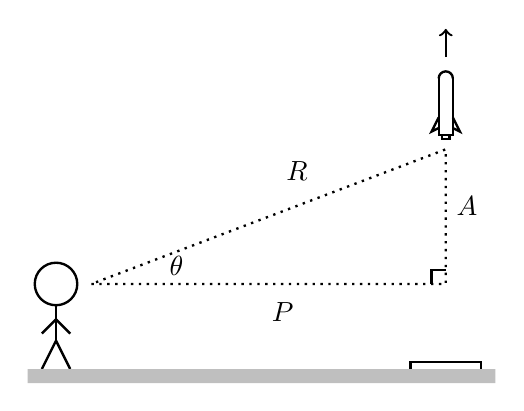
\begin{tikzpicture}[scale=0.9]
	% Rocket
	\draw[line width=0.03cm] (-0.1,4.1) -- (-0.1,3.3) -- (0.1,3.3) -- (0.1,4.1);
	\myarc{line width=0.03cm}{0}{4.1}{0.1}{0}{180};
	\draw[line width=0.03cm] (-0.05,3.3) -- (-0.05,3.25) -- (0.05,3.25) -- (0.05,3.3);
	\draw[line width=0.03cm] (-0.1,3.55) -- (-0.2,3.35) -- (-0.1,3.4);
	\draw[line width=0.03cm] (0.1,3.55) -- (0.2,3.35) -- (0.1,3.4);
	\draw[line width=0.03cm,->] (0,4.4) -- (0,4.8);
	% Person
	\draw[line width=0.03cm] (-5.5,1.2) circle (0.3); % head
	\draw[line width=0.03cm] (-5.5,0.9) -- (-5.5,0.4); % body
	\draw[line width=0.03cm] (-5.5,0.4) -- (-5.3,0); % left leg
	\draw[line width=0.03cm] (-5.5,0.4) -- (-5.7,0); % right leg
	\draw[line width=0.03cm] (-5.5,0.7) -- (-5.3,0.5); % left arm
	\draw[line width=0.03cm] (-5.5,0.7) -- (-5.7,0.5); % right arm
	% Platform
	\draw[line width=0.03cm] (-0.5,0) -- (-0.5,0.1) -- (0.5,0.1) -- (0.5,0);
	% Ground
	\draw[line width=0.01cm,fill=gray!50,draw=none] (-5.9,0) -- (-5.9,-0.2) -- (0.7,-0.2) -- (0.7,0) -- (-5.9,0);
	% Triangle
	\draw[line width=0.03cm,dotted] (-5,1.2) -- (0,1.2) -- (0,3.1) -- (-5,1.2);
	\draw[line width=0.03cm] (-0.2,1.2) -- (-0.2,1.4) -- (0,1.4);
	% Labels
	\node at (-3.8,1.45) {$\theta$};
	\node at (-2.3,0.8) {$P$};
	\node at (0.3,2.3) {$A$};
	\node at (-2.1,2.8) {$R$};
	\end{tikzpicture}
	\]
We also know\dots
	\[
	\begin{aligned}
	P&= 810 \text{ ft \quad *Constant} \\[0.2cm]
	\theta&= 60^\circ \cdot \tfrac{\pi}{180}= \dfrac{\pi}{3} \\[0.2cm]
	\dfrac{d\theta}{dt}&= 10^\circ \cdot \tfrac{\pi}{180}= \dfrac{10\pi}{180}= \dfrac{\pi}{18}
	\end{aligned}
	\]
We want to know the speed of the rocket, which will be the same as $\dfrac{dA}{dt}$---the rate of change of the height of the rocket above the ground. Using trigonometry, we know\dots
	\[
	\begin{aligned}
	\tan \theta= \dfrac{A}{P} \\
	P \tan \theta= A
	\end{aligned}
	\]
We can substitute $P$ because it is constant with respect to time. But then\dots
	\[
	\begin{gathered}
	A= 810 \tan \theta \\[0.2cm]
	\dfrac{d}{dt}\, A= \dfrac{d}{dt} \,( 810 \tan \theta ) \\[0.2cm]
	\dfrac{dA}{dt}= 810 \sec^2 \theta \cdot \dfrac{d\theta}{dt}
	\end{gathered}
	\]
But $\theta= \frac{\pi}{3}$ and $\tfrac{d\theta}{dt}= \tfrac{\pi}{18}$. Therefore, we have\dots
	\[
	\dfrac{dA}{dt}= 810 \sec^2 \left( \tfrac{\pi}{3} \right) \cdot \dfrac{\pi}{18}= \cancel{810}^{\,9^2 \cdot 10} \cdot 2^2 \cdot \dfrac{\pi}{9 \cdot 2}= (9^{\cancel{2}} \cdot 10) \cdot 2^{\cancel{2}} \cdot \dfrac{\pi}{\cancel{9} \cdot \cancel{2}}= 9 \cdot 10 \cdot 2 \cdot \pi= \boxed{180 \pi} \approx 565.487
	\] \pspace
Therefore, the rocket is rising at a rate of approximately 565.487~ft per second, i.e. 385.559~mph.}



% Question 6
\newpage
\question[15] A function and its derivatives are given below.
	\[
	f(x)= \dfrac{x^2 + 9}{x}, \qquad f'(x)= \dfrac{x^2 - 9}{x^2}, \qquad f''(x)= \dfrac{18}{x^3}
	\]
Showing all your work, use the information above to answer the questions below. 
        \begin{enumerate}[(a)]
        \item Find and classify the critical values (if any) for $f(x)$ as local maxima, local minima, or neither. \par\vspace{0.1cm}

        \wsol{\itshape\scriptsize Critical values are where $f'(x)$ is undefined or $0$. We can see that $f'(x)$ is undefined at $x= 0$. Setting $f'(x)= 0$, we have $\dfrac{x^2 - 9}{x}= 0$. But then $x^2 - 9= 0$, so that $(x - 3)(x + 3)= 0$. But then either $x - 3= 0$, which implies $x= 3$, or $x + 3= 0$, which implies that $x= -3$. Therefore, the critical values are $x= -3, 0, 3$. We can classify these values as maxima, minima, or neither using the first derivative test:
		\[
		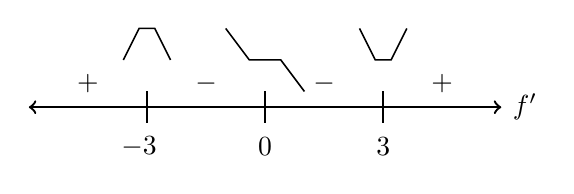
\begin{tikzpicture}
		\node at (3.3,0) {$f'$};
		\draw[line width=0.03cm,<->] (-3,0) -- (3,0);
		\draw[line width=0.02cm] (-1.5,-0.2) -- (-1.5,0.2);
		\draw[line width=0.02cm] (0,-0.2) -- (0,0.2);
		\draw[line width=0.02cm] (1.5,-0.2) -- (1.5,0.2);
		
		\node at (-1.6,-0.5) {$-3$};
		\node at (0,-0.5) {$0$};
		\node at (1.5,-0.5) {$3$};
		
		\node at (-2.25,0.3) {$+$};
		\node at (-0.75,0.3) {$-$};
		\node at (0.75,0.3) {$-$};
		\node at (2.25,0.3) {$+$};
		
		\draw[line width=0.02cm] (-1.8,0.6) -- (-1.6,1) -- (-1.4,1) -- (-1.2,0.6);
		
		\draw[line width=0.02cm] (-0.5,1) -- (-0.2,0.6) -- (0.2,0.6) -- (0.5,0.2);
		
		\draw[line width=0.02cm] (1.2,1) -- (1.4,0.6) -- (1.6,0.6) -- (1.8,1);
		\end{tikzpicture}
		\]
	If we used the second derivative test, observe that $f''(-3) < 0$ and $f''(3) > 0$. We can see that $x= -3$ is a local maximum and $x= 3$ is a local minimum. Note that $x= 0$ is not in the domain of $f(x)$, so it cannot be a local maxima or a local minima. Therefore, we have\dots
		\[
		\boxed{%
		\begin{aligned}
		x= -3 &: \text{local maxima} \\
		x= 0 &: \text{neither} \\
		x= 3 &: \text{local minima}
		\end{aligned}
		}
		\]
	}

        \item Find the intervals where $f(x)$ is increasing and find the intervals where $f(x)$ is decreasing, if any such intervals exist. \par\vspace{0.1cm}

        \wsol{\itshape\scriptsize We know that $f(x)$ is increasing when $f'(x) > 0$ and that $f(x)$ is decreasing when $f'(x) < 0$. But observe using a sign-line for $f'(x)$ that was constructed in (a), we have\dots
		\[
		\boxed{
		\begin{aligned}
		\text{Increasing} &: (-\infty, -3) \cup (3, \infty) \\
		\text{Decreasing}&: (-3, 0) \cup (0, 3)
		\end{aligned}
		}
		\]
        }

        \item Find the intervals where $f(x)$ is concave and find the intervals where $f(x)$ is convex, if any such intervals exist. \par\vspace{0.1cm}

        \wsol{\itshape\scriptsize We know $f(x)$ is concave when $f''(x) < 0$ and $f(x)$ is convex when $f''(x) > 0$. But then $f(x)$ is clearly concave when $x < 0$ and convex when $x > 0$. We can also create a sign-line for $f''(x)$: the only value where $f''(x)$ is undefined or 0 is at $x= 0$ (where $f''(x)$ is undefined). 
        		\[
		\begin{tikzpicture}
		\node at (2.3,0) {$f''$};
		\draw[line width=0.03cm,<->] (-2,0) -- (2,0);
		\draw[line width=0.02cm] (0,-0.2) -- (0,0.2);
		
		\node at (0,-0.5) {$0$};
		\node at (-1,0.3) {$-$};
		\node at (1,0.3) {$+$};
		\end{tikzpicture}
		\]
	Therefore, we have\dots
		\[
		\boxed{
		\begin{aligned}
		\text{Concave} &: (-\infty, 0) \\
		\text{Convex}&: (0, \infty)
		\end{aligned}
		}
		\]
	}

        \item Find any inflection points for $f(x)$, if any. \par\vspace{0.1cm}

        \wsol{\itshape\scriptsize An inflection point is a point on the graph of $f(x)$ where $f''(x)$ changes sign. From our work from (c), this can only be at $x= 0$. However, $x= 0$ is not in the domain of $f(x)$, so there is no corresponding point on the graph of $f(x)$. Therefore, $f(x)$ has no point of inflection. 
		\[
		\boxed{
		\begin{aligned}
		\text{No point of inflection}
		\end{aligned}
		}
		\]
	}
        \end{enumerate}

\end{questions}
\end{document}